\documentclass{article}
\usepackage[utf8]{inputenc}
\usepackage{pgfplots}
\usepackage[utf8]{inputenc}
\usepackage[shortlabels]{enumitem}
\usepackage{amsmath} 
\usepackage{gensymb}
\usepackage{geometry}
\usepackage{listings}
\usepackage{xcolor}
\usepackage{pgfplots}
\usepackage{pgfplotstable}
\pgfplotsset{compat=1.7}
\usepackage{tikz}
\geometry{
 a4paper,
 total={170mm,257mm},
 left=20mm,
 top=20mm,
}
\title{Assignment: Data Organization}
\author{Andy Yan}
\date{September 2022}

\begin{document}

\maketitle

\section{Ungrouped Data}
35.6,  66.9,  57.4,  73.3,  70.7,  48.6,  47.5,  68.8,  39.3,  40.8,  52.6,  55.4,  43.9,  58.8,
62.2,  68.3,  70.1,  64.9,  64.2,  45.7,  49.2,  56.4,  63.7,  39.8,  64.5,  60.0,  58.1,  45.9

\section{Grouped Data}
\begin{center}
\def\arraystretch{1}
{\setlength{\tabcolsep}{5em}
\begin{tabular}{| c | c | c |} 
\hline
\multicolumn{2}{|c|}{Grouped Frequency Distribution Table} \\
 \hline
   Class Interval & Frequency\\ [1ex] 
 \hline
35.6 - 41.1 & 4\\
 \hline
42.1 - 47.6	& 4\\
 \hline
48.6 - 54.1	& 3\\
 \hline
55.1 - 60.6	& 6\\
 \hline
61.6 - 67.1	& 6\\
 \hline
 68.1 - 73.6	& 5\\
 \hline
  \textbf{Total:} & \textbf{28}\\
  \hline
\end{tabular}}
\end{center}

\section{Histogram}
\begin{center}
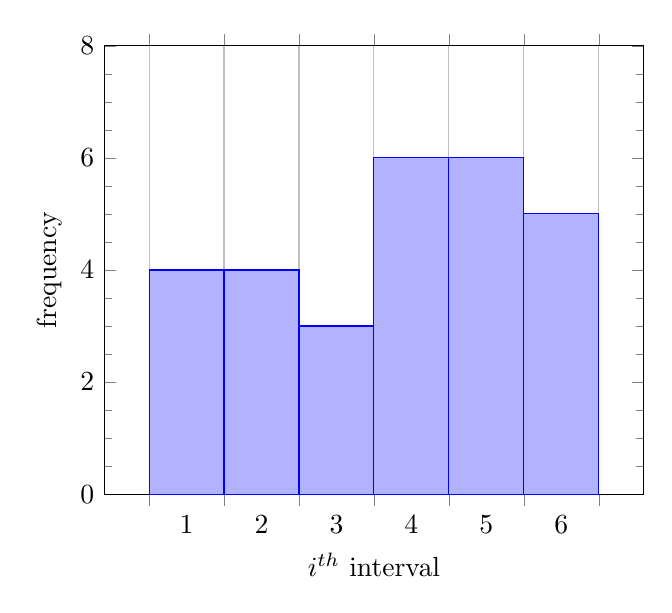
\begin{tikzpicture}

\begin{axis}[ybar interval, ymax=8,ymin=0, minor y tick num = 3 ,
    xlabel=\(i^{th}\) interval,
	ylabel=frequency
    ]
\addplot coordinates { (1, 4) (2, 4) (3, 3) (4, 6) (5, 6) (6, 5) (7, 5) };
\end{axis}

\end{tikzpicture}
\end{center}

\section{Cumulative Relative Frequency Table}
\begin{center}
\def\arraystretch{1}
\begin{tabular}{| c | c | c | c | c |} 
\hline
\multicolumn{5}{|c|}{Cumulative Relative Frequency Table} \\
 \hline
   Class Interval & Frequency & Cumulative Frequency & Relative Frequency & Cumulative Relative Frequency\\
 \hline
35.6 - 41.1 & 4 & 4 & 0.1429 & 0.1429\\
 \hline
42.1 - 47.6	& 4 & 8 & 0.1429 & 0.2857\\
 \hline
48.6 - 54.1	& 3 & 11 & 0.1070 & 0.3929\\
 \hline
55.1 - 60.6	& 6 & 17 & 0.2143 & 0.6071\\
 \hline
61.6 - 67.1	& 6 & 23 & 0.2143 & 0.8217\\
 \hline
 68.1 - 73.6	& 5 & 28 & 0.1786 & 1\\
  \hline
\end{tabular}
\end{center}

\section{Sorted Data (Ascending)}
35.6,  39.3,  39.8,  40.8,  43.9,  45.7,  45.9,  47.5,  48.6,  49.2,  52.6,  55.4,  56.4,  57.4,  58.1,  58.8,  60.0,  62.2,  63.7,  64.2,  64.5,  64.9,  66.9,  68.3,  68.8,  70.1,  70.7,  73.3

\section{Cumulative Relative Frequency Graph}
\[PR = b/n \cdot 100\%\]
\textbf{Graph 1}

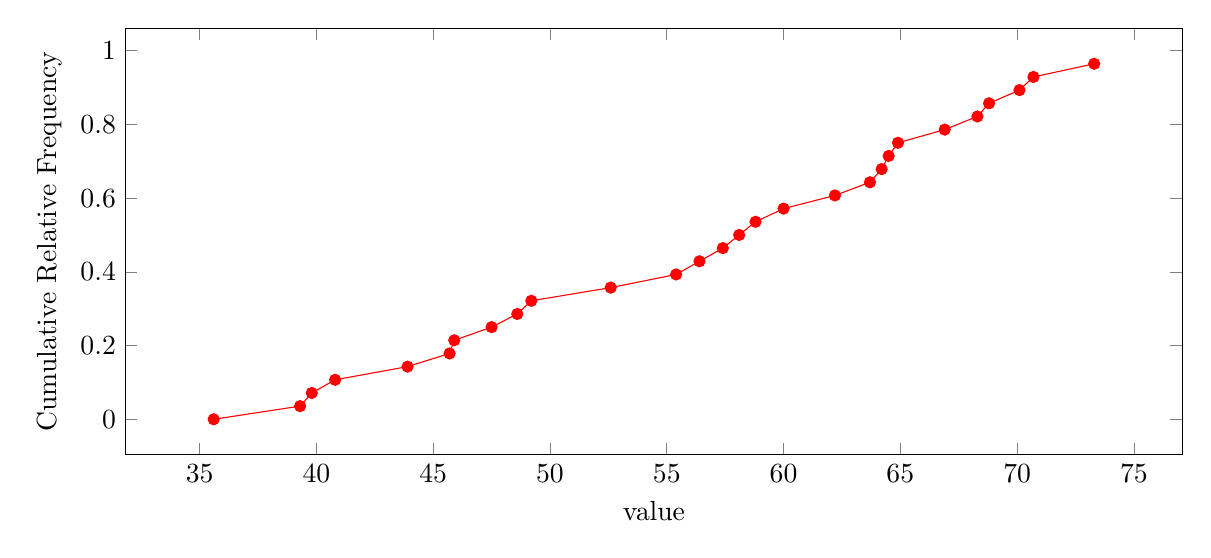
\begin{tikzpicture}
\begin{axis}[
	xlabel=value,
	ylabel=Cumulative Relative Frequency,
	width=15cm,height=7cm,
    legend style={at={(0.0,.91)},anchor=west}
    ]

% Add values and attributes for the first plot
\addplot[color=red,mark=*] coordinates {
(35.6, 0.0)
(39.3, 0.03571428571428571)
(39.8, 0.07142857142857142)
(40.8, 0.10714285714285714)
(43.9, 0.14285714285714285)
(45.7, 0.17857142857142858)
(45.9, 0.21428571428571427)
(47.5, 0.25)
(48.6, 0.2857142857142857)
(49.2, 0.32142857142857145)
(52.6, 0.35714285714285715)
(55.4, 0.39285714285714285)
(56.4, 0.42857142857142855)
(57.4, 0.4642857142857143)
(58.1, 0.5)
(58.8, 0.5357142857142857)
(60.0, 0.5714285714285714)
(62.2, 0.6071428571428571)
(63.7, 0.6428571428571429)
(64.2, 0.6785714285714286)
(64.5, 0.7142857142857143)
(64.9, 0.75)
(66.9, 0.7857142857142857)
(68.3, 0.8214285714285714)
(68.8, 0.8571428571428571)
(70.1, 0.8928571428571429)
(70.7, 0.9285714285714286)
(73.3, 0.9642857142857143)

};

\end{axis}
\end{tikzpicture}

\section{Questions}
\indent 1. From the above cumulative relative frequency diagram, what a percent of data is greater than 50? [2A]
\\
\\
There are 18 values greater than 18.
\[18/28 \cdot 100\% \approx 64.29\%\]
\textbf{Therefore, 64.29\% of the data is greater than 50.}

\\
\\
2. From the above cumulative relative frequency diagram, what value is the 40th percentile?  [2A]
\\
\\
From the diagram we can see that at y-value 0.4, we approximate a value 54.3. This means the value 54.3 is greater than 40\% of the data.

To find the exact value we can do this:
\[40\% \cdot (28 + 1) = 11.6\]
\[P_{40} = 52.6 + 0.6(55.4-52.6) = 54.28\]

\textbf{Therefore, the value of the 40th percentile is 54.28.}

\end{document}
